\documentclass[10pt,a4paper]{report}
\usepackage[utf8]{inputenc}
\usepackage[german]{babel}
\usepackage[T1]{fontenc}
\usepackage{amsmath}
\usepackage{amsfonts}
\usepackage{amssymb}
\usepackage{graphicx}
\usepackage{listings}
\usepackage[left=2cm,right=2cm,top=2cm,bottom=2cm]{geometry}
\title{LPR-P2 Doku 2019}

\begin{document}
%Julia
\chapter{Material und Methoden}
Die Entwicklung des Emotionserkennungsspiel ist in drei Bereichen geteilt:
die graphische Benutzeroberfl\"{a}che, die dahinter steckende Logik bzw. das
Neuronale Netz, das f\"{u}r die Emotionserkennung zust\"{a}ndig ist und die Schnittstelle
zwischen beiden. Im Folgenden werden die Methoden der einzelnen Bestandteile
des Programms beschrieben. 
\section{Neuronale Netze}
\label{subsec:statistical-summaries}
Auf Grund seiner h\"{o}heren Geschwindigkeit und gro{\ss}en Anzahl von verschiedenen
bereitgestellten Bibliotheken gilt Python als eine der besten Programmiersprachen
f\"{u}r die Entwicklung einer K\"{u}nstlichen Intelligenz-basierten Software.
Python wird in Kombination mit dem Deep Learning Framework  \textit{TensorFlow} angewendet, um das Netz \"lehren\" und seine Ergebnisse interpretieren zu k\"{o}nnen.
Bei diesem Projekt wurden die Python Version 3.6 und die TensorFlow Version
1.7 verwendet.
Als Vorlage diente ein Beispielskript \cite{LeweOhlsenGit}, das ein Videosignal \"{u}ber die Webkamera
empf\"{a}ngt, das Video dann in einzelne Bilder (Frames) zerteilt und jedes Bild
nach Emotionen untersucht. Das Skript wurde w\"{a}hrend des Laborpraktikums
umgebaut und an die Benutzeroberfl\"{a}che und die Schnittstellen angepasst.\newline
Um die einzelne Bilder zu bewerten reicht das neuronale Netz allein nicht aus. Man
ben\"{o}tigt auch ein Framework, das Bildverarbeitungs-Algorithmen zur Verf\"{u}gung
stellt. Ein solches Framework ist OpenCV, da es sich gut mit Python kompilieren l\"{a}sst.
Zur Verf\"{u}gung standen drei bereits trainierten neuronalen Netze bzw. Modelle:
\begin{itemize}
\item[-]  FER2013 \cite{IasGoodefellow}
\item[-] CK+
\item[-] FERPlus
\end{itemize}
 

Eines dieser Modelle  bindet man in das Skript ein, um auf der Basis des ausgew\"{a}hlten Modells die Emotionserkennung zu erm\"{o}glichen. Bei dem im Emotionserkennungsspiel verwendeten Datensatz 
handelt es sich um den FERPlus-Datensatz. 
 \cite{LeweOhlsen} Der Datensatz wurde
von einer Forschungsgruppe bei Microsoft entwickelt. Er unterscheidet sich
von seinem Vorg\"{a}nger FER2013 im genaueren Crowdsourcing f\"{u}r den Tagging-
Vorgang.
 \cite{RamakrishnanPandeyKarmakarSaha} 
Dieser Datensatz verf\"{u}gt \"{u}ber sieben Emotionsklassen: Wut, Ekel,
Angst, Freude, Trauer, \"{u}berraschung und neutrale Emotion.
Im Gegensatz zum Beispielsskript, empf\"{a}ngt das f\"{u}r das Spiel entwickelte Skript 
keinen Stream von der Webkamera, sondern bekommt von der Benutzeroberfl\"{a}che
ein Ordnerverzeichnis \"{u}bergeben. In dem Ordner befinden sich Bilder, die bereits
aus dem Videostream ausgeschnitten worden sind. 
%Die Bilder werden nach der Erkennung gel\"{o}scht. Dieser Satz ist in der aktuellen Programmlogik nicht mehr g\"{u}ltig.
In einem Ordner sollen Bilder mit der gleichen Emotion abgespeichert werden. Die Bilder nacheinander werde
eingelesen.
Zun\"{a}chst wird \"{u}berpr\"{u}ft, ob auf dem Bild ein Gesicht gefunden bzw.
erkannt werden kann. Laut den Spielregeln darf es nur einen Spieler geben,
daher liefert das Skript eine bestimmte Meldung zur\"{u}ck, sollte die Neuronale Netz mehr als ein Gesicht oder kein
Gesicht erkennen. Falls aber
tats\"{a}chlich ein Gesicht erkannt wird, geht das Spiel weiter. Das Gesicht auf
jedem Bild wird nach Emotionen Untersucht. Das Ergebnis wird auf der Kommandozeile
in Form eines Feldes ausgegeben, in dem auf der ersten Position das
Index von der Emotion steht, die am wahrscheinlichsten erkannt wurde.
%David
\chapter{Klassenbeschreibung}
\section{Emotionserkennung – Zusammenspiel der verschiedenen Klassen}
Die Erkennung einer Emotion anhand der zur Verf\"{u}gung gestellten Bilder erfolgt durch ein Zusammenspiel der Klassen \textit{PrepareModel} und \textit{EmotionTableInterpreter}. Das Starten des Python-Prozesses zur Ermittlung der erkennbaren Emotionen liegt im Aufgabenbereich der \textit{PrepareModel}-Klasse. Des Weiteren startet \textit{PrepareModel} die Auswertung der vom Python-Prozess zur\"{u}ckgegeben Werte mittels der \textit{EmotionTableInterpreter}-Klasse. Ziel ist es, die am deutlichsten erkannte Emotion heraus zu filtern. Der Interpreter bef\"{u}llt danach das Attribut \textit{ReturnObject} der \textit{PrepareModel}-Klasse mit Informationen bez\"{u}glich der Auswertung. Dieses Objekt dient zur \"{u}bermittlung und zur Bewertung der enthaltenen Informationen.
\section{Beschreibung der einzelnen Klassen und deren Funktionalit\"{a}ten}
\subsection{PrepareModel}
\subsubsection{PrepareModel – Konstruktor}
Im Konstruktor der Klasse \textit{PrepareModel} wird eine Variable der Klasse \textit{Process} definiert und mit den entsprechenden Start-Informationen bef\"{u}llt. Darunter befindet sich beispielsweise der Pfad zu dem auszuf\"{u}hrenden Python-Script oder auch der Pfad zu den auszuwertenden Bildern. Final wird die Funktion \textit{StartEmoRecTableInterpreter} ausgef\"{u}hrt.
\subsubsection{StartEmoRecTableInterpreter}
In dieser Funktion wird eine neue Instanz der Klasse \textit{EmotionTableInterpreter} erstellt und dabei die im Konstruktor definierte Prozess-Variable und das Attribut \textit{ReturnObject} \"{u}bergeben.
\subsubsection{GetReturnObject}
\textit{GetReturnObject} gibt das Attribut \textit{ReturnObject} der Klasse \textit{PrepareModel} zur\"{u}ck, welches w\"{a}hrend der Auswertung bef\"{u}llt wurde. 
\subsection{ReturnObject}
Hierbei handelt es sich um eine Klasse, die zur R\"{u}ckgabe der durch die Auswertung erlangten Informationen dient. Das Objekt umfasst beschreibende und prozentuale Informationen zur erkannten Emotion. Des Weiteren verf\"{u}gt es \"{u}ber eine Enumeration, welche den Typ der R\"{u}ckgabe definiert. Dieser Typ gibt Auskunft \"{u}ber die Auswertbarkeit der in dem Objekt enthaltenen Informationen.
\subsection{EmotionTableInterpreter}
\subsubsection{EmotionTableInterpreter – Konstruktor}
Dem Konstruktor der \textit{EmotionTableInterpreter}-Klasse werden sowohl die Prozess-Variable, sowie das R\"{u}ckgabe-Objekt der \textit{PrepareModel}-Klasse \"{u}bergeben. Der Prozess wird innerhalb des Konstruktors gestartet und dessen Ausgabe mit Hilfe von regul\"{a}ren Ausdr\"{u}cken verarbeitet. Bevor die Auswertung der Prozessausgabe durch die \textit{Evaluate}-Funktion erfolgt, wird zuerst die Auswertbarkeit der Daten \"{u}berpr\"{u}ft. Enth\"{a}lt eines der \"{u}bergebenen Bilder mehr als ein erkanntes Gesicht wird die Auswertung nicht gestartet und entsprechende Informationen mit Hilfe des \textit{ReturnObjects} zur\"{u}ckgegeben. Enthalten die Bilder kein einziges Gesicht erfolgt ebenfalls keine Auswertung und das R\"{u}ckgabe-Objekt ist vom Typ \textit{„NoFaceDetected“}. Die Auswertung durch \textit{Evaluate} startet, wenn in einer Bilderserie mindestens ein Bild genau ein Gesicht enth\"{a}lt und alle anderen Bilder kein Gesicht oder maximal ein Gesicht aufweisen.
\subsubsection{Evaluate}
Die Ausgabe des Python-Prozesses liefert Informationen \"{u}ber die im Bild erkannten Emotionen. Erkennbar sind Wut, Ekel, Angst, Fr\"{o}hlichkeit, Traurigkeit, ein \"{u}berraschter und ein neutraler Gesichtsausdruck. Die Prozess-Ausgabe pro Bild liefert f\"{u}r jede der obengenannten Emotionen eine Gewichtung. Durch die Funktion \textit{Evaluate} wird von jedem bewerteten Bild die h\"{o}chst gewichtete Emotion dem Attribut \textit{hdEmoCollection} der Klasse \textit{EmotionTableInterpreter} hinzugef\"{u}gt. Bei \textit{hdEmoCollection} handelt es sich um ein Feld des Typs \textit{Dictornary}, welches sich als Sammlung mehrerer Schl\"{u}ssel-Wert-Paare definiert. Bei der Zuordnung der sogenannten „\textit{highest detected emotion“} durch die \textit{Evaluate}-Funktion wird wie folgt vorgegangen. Die Beschreibung der Emotion (bspw. \textit{„Fear“}) dient als Schl\"{u}ssel eines \textit{hdEmoCollection}-Schl\"{u}ssel-Wert-Paares und die Gewichtung der signifikantesten Emotion als Wert. Wird die Emotion \textit{„Fear“} mehrmals pro Auswertung erkannt erh\"{o}ht dies den Wert des \textit{hdEmoCollection}-Elements um die jeweilige Gewichtung. So liefert die Funktion Evaluate eine Zusammenfassung der am besten erkannten Emotionen mit den aufsummierten Gewichtungen. (Siehe Abbildung \ref{fig:VisualisierungEvaluation})
 \begin{figure}
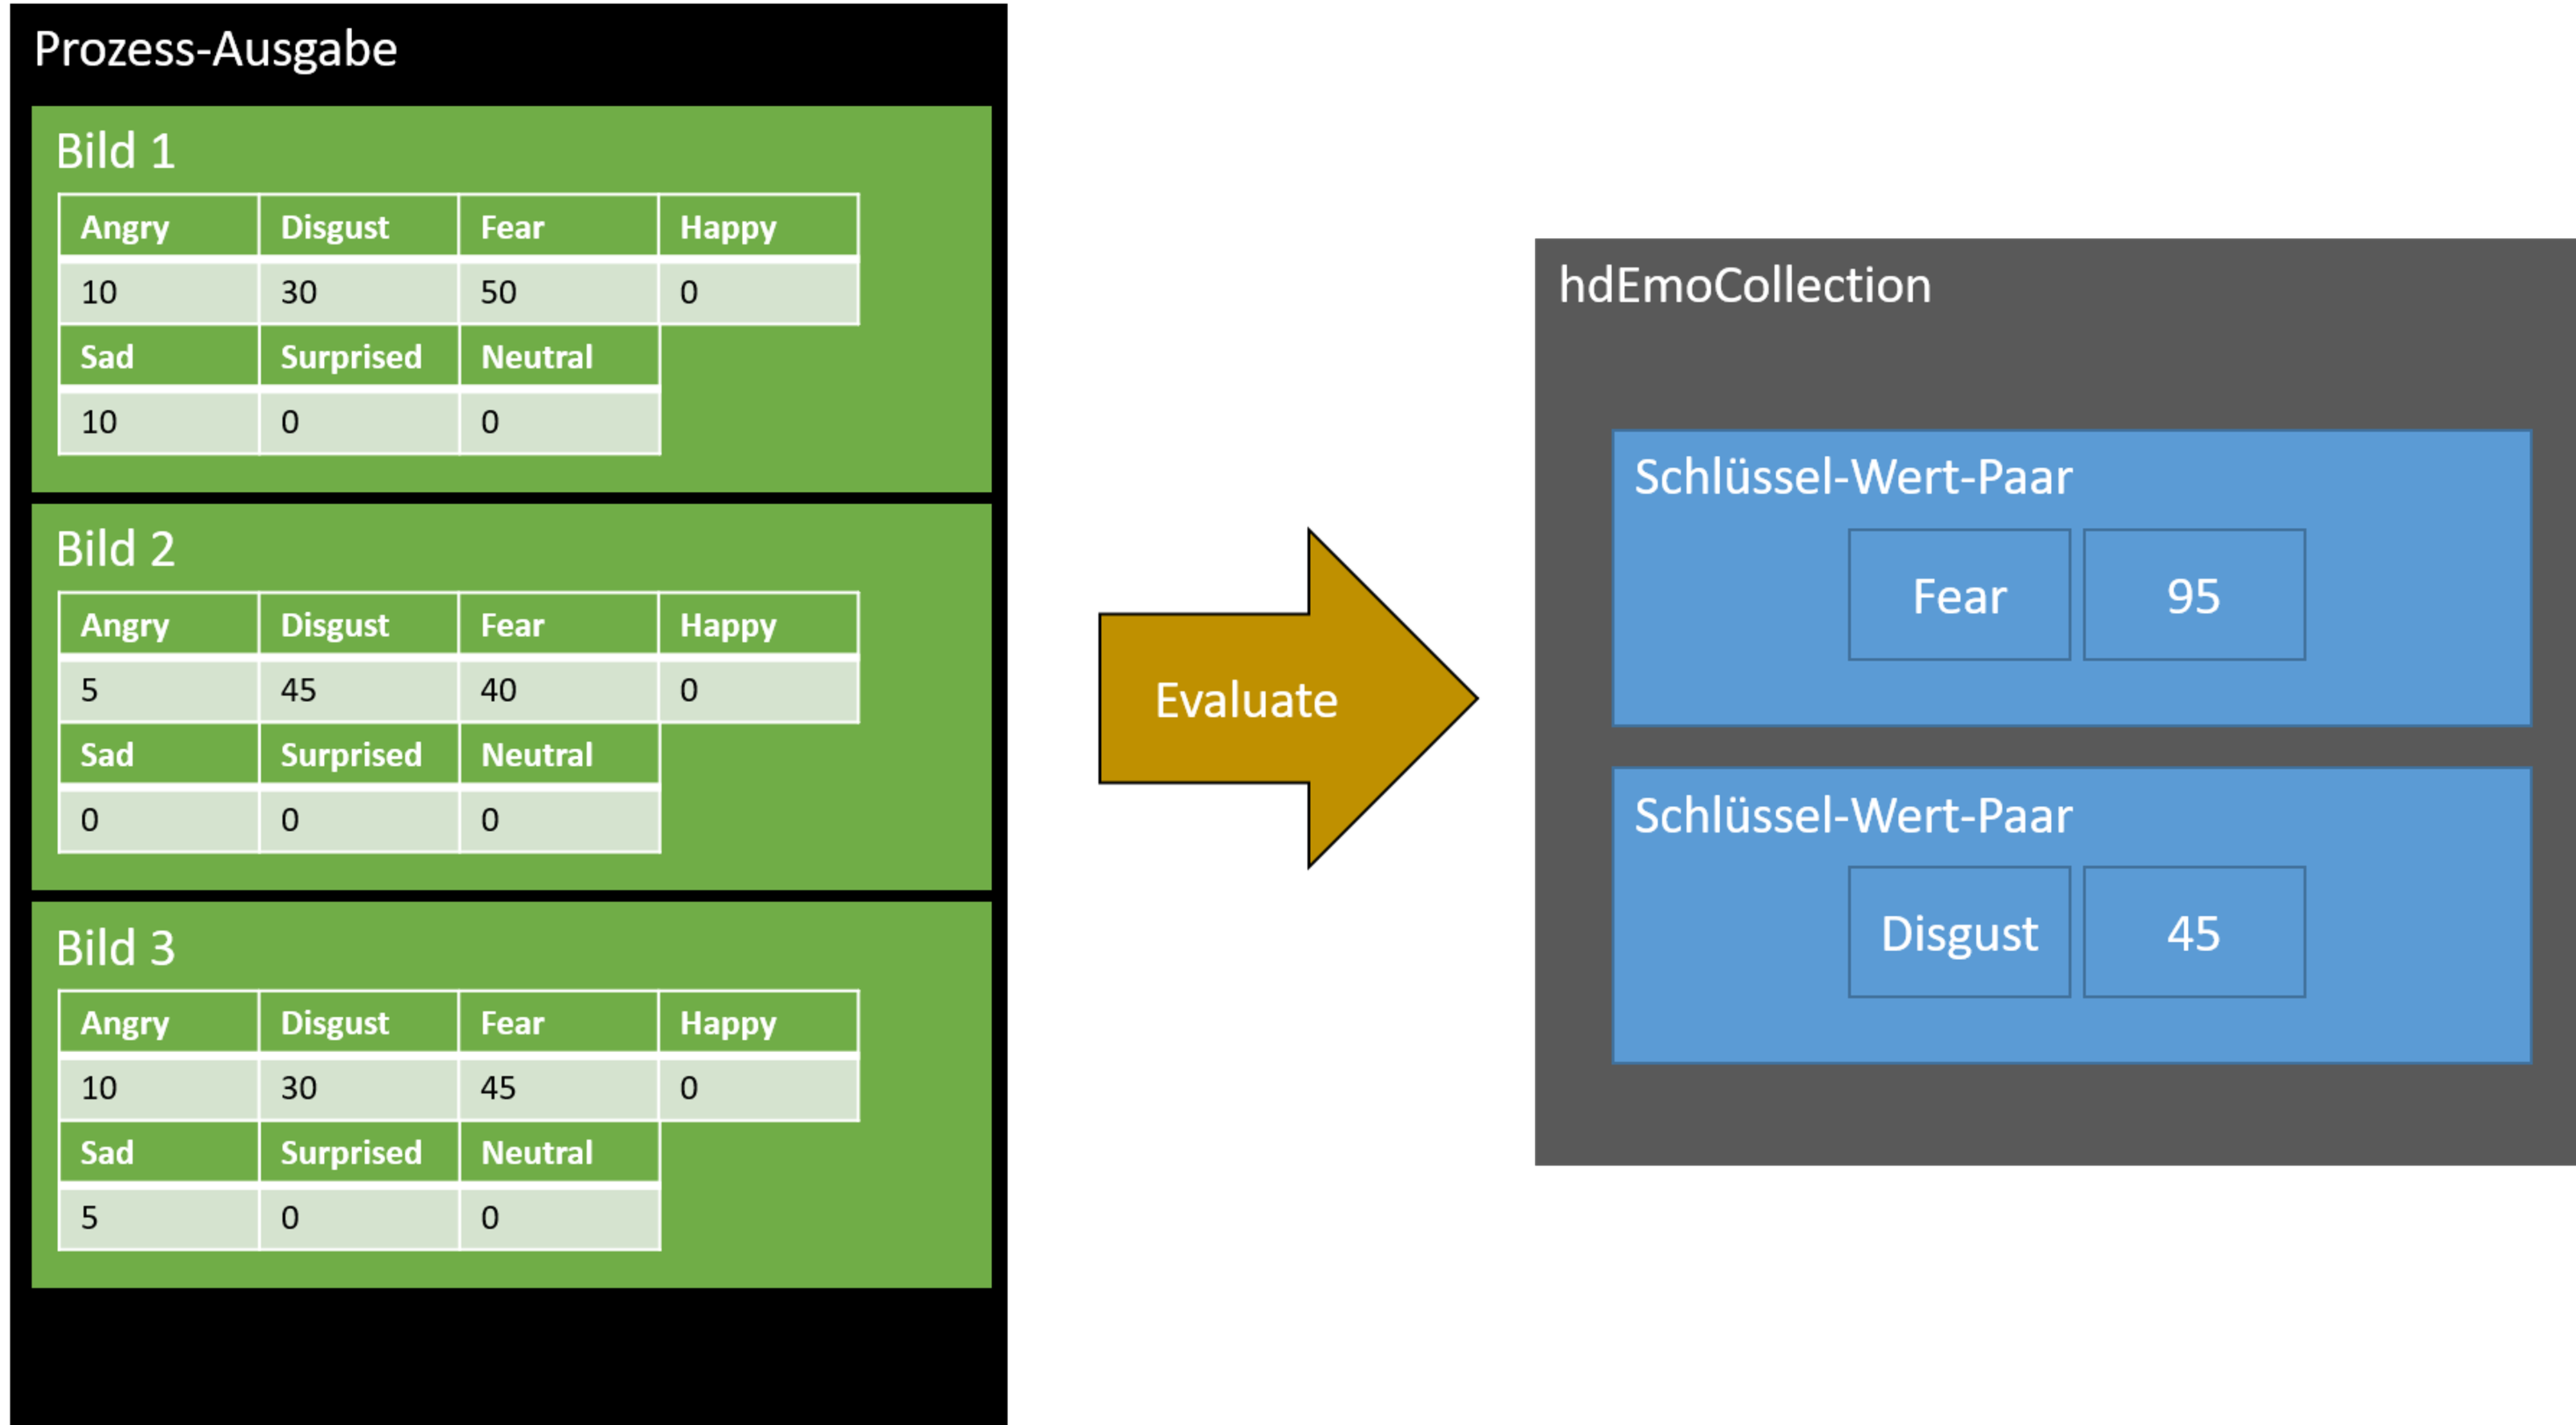
\includegraphics[scale=0.27]{Evaluate_Veranschaulichung.pdf}
 \caption{Visualisierung des Auswertungsvorgangs}
 \label{fig:VisualisierungEvaluation}
 \end{figure}
\subsubsection{GetEmotion}
Diese Funktion liefert das Schl\"{u}ssel-Wert-Paar der \textit{hdEmoCollection}, welches den h\"{o}chsten Wert und somit auch die h\"{o}chste Gewichtung enth\"{a}lt. Tritt der Fall ein, dass die Emotion \textit{„Neutral“} und eine beliebig andere Emotion, beispielsweise \textit{„Happy“}, den gleichen und h\"{o}chsten Wert aufweisen, liefert die \textit{GetEmotion}-Funktion \textit{„Happy“}. Bei \textit{„–Neutral“} handelt es sich um keine vom Benutzer zu fordernde Emotion und somit rechtfertigt sich diese Sonderregelung.

%Lukas
\section{Regul\"{a}re Ausdr\"{u}cke in der Ergebniserkennung}
In der Klasse \textit{EmotionTableInterpreter} werden drei Regul\"{a}re Ausdr\"{u}cke benutzt, um die Ergebnisse des Python-Skripts, die als Konsolenausgabe vorliegen, in das Programm zu importieren. Zwei dieser Ausdr\"{u}cke werden zur Erkennung verwendet, der dritte l\"{o}scht Steuerzeichen, die im Eingabestring m\"{o}glicherweise vorhanden sind. Die \texttt{System.Text.RegularExpressions}-Bibliothek bindet die Funktionalit\"{a}t zur Verwendung der Regul\"{a}ren Ausdr\"{u}cke ein.
\subsection{Begriffsdefinitionen}
\begin{itemize}
\item[-] Eingabestring: String, dessen Inhalt auf \textit{Matches} durchsucht wird.
\item[-] Match (\textit{plural: Matches}): Teilstring(s) des \textit{Eingabestrings}, der mit dem \textit{Pattern} \"{u}bereinstimmt.
\item[-] Pattern: Regul\"{a}rer Ausdruck
\item[-] Subpattern: Teil eines Regul\"{a}ren Ausdrucks, der benannt wird, um leichter auf ihn zugreifen zu k\"{o}nnen. Einzelne Subpattern k\"{o}nnen auch gematcht werden. 
\end{itemize}
\subsection{Regul\"{a}re Ausdr\"{u}cke f\"{u}r die Prozessausgabe}
Die einzelnen Pattern zur Auswertung der Ausgabe werden im Folgenden erkl\"{a}rt.
\subsubsection{patternFaceFoundCount}
Das Pattern \texttt{(Faces found:  (?<FacesFoundCount>[0-9]*))\{1\}} hat den Zweck, die Anzahl der erkannten Gesichter in einem Bild auszulesen. Das Subpattern \texttt{((?<FacesFoundCount>[0-9]*))\{1\}} mit dem Namen \textit{FacesFoundCount} hat als Match eine Zahl aus dem Intervall $\left[0;9\right] \in \mathbb{N}$ und gibt diese bei einem Aufruf zur\"{u}ck. Dieser Wert wird verwendet, um zu entscheiden, ob die vom Modell erzeugten Daten im \textit{EmotionTableInterpreter} ausgewertet werden sollen, oder nicht. Im Abschnitt \"PrepareModel - Konstruktor\" findet sich eine genauere Erkl\"{a}rung.
\subsubsection{patternArray}
Der erste Teil des Patterns hei{\ss}t\textit{SinglePicOutput}. Dieses Subpattern umfasst das gesamte Pattern und soll den 
Zugriff auf den Gesamtoutput eines einzelnen Bildes vereinfachen. Direkt nach der Benennung des Subpatterns beginnt 
das erste Array, dessen Zahl auf dem Index 0 die erkannte Emotion anzeigt. Auf diese Zahl kann sp\"{a}ter mit dem Subpattern 
\texttt{(ar+ay([(?<HighestEmotionIndex>[0-6])} zugegriffen werden.  Ebenso liefert es so den Index im zweiten Array, 
welches die Gewichtung der vom Netz erkannten Emotion enth\"{a}lt. Die restlichen sechs Elemente des Arrays werden nicht in 
einem Subpattern erfasst. Das Pattern muss sie trotzdem erkennen, da  sonst die Erkennung des zweiten Arrays 
schwieriger ist. Dies erfolgt mit dem folgenden Abschnitt: \texttt{([,][ ]*[0-6])*][, dtype=int[32|64]*]*)[,][]*}. Der Abschnitt 
erkennt eine unbekannte Anzahl an Zahlen aus dem Intervall $\left[0;6\right] \in \mathbb{N}$, denen jeweils ein Komma 
folgt. Zwischen dem Komma der letzten Zahl und der n\"{a}chsten Zahl kann sich wiederum eine unbekannte Anzahl an 
Leerzeichen befinden.
Die Gewichtungen im zweiten Array, genannt \texttt{(?<EmotionWeightArray>} werden als Flie{\ss}kommazahlen 
dargestellt. Niedrige Wahrscheinlichkeiten werden mit Hilfe der Exponentialschreibweise ausgegeben. Dies kann zu Zahlen 
wie \texttt{2.8267652e-05} (=> \texttt{2.8267652 $\cdot$ 10$^{-5}$}) f\"{u}hren. Da diese Zahlen potentiell alle das Gewicht 
f\"{u}r die h\"{o}chste erkannte Emotion darstellen k\"{o}nnen, werden sie alle getrennt mit Hilfe von eigenen Subpattern erkannt, 
damit einfach auf sie zugegriffen werden kann. Dies wird im Abschnitt \"Ablauf\" eingehender besprochen. Die Subpattern 
f\"{u}r die Flie{\ss}kommazahlen sind gleich aufgebaut. \texttt{(?<EmotionWeightArray2>[0-9]*[.]*[0-9]*[e]*[-|+]*[0-9]*)} 
erkennt die Gewichtung an der dritten Stelle im Array. Die Zahl ist in sechs Bereiche unterteilt, die jeweils den Anteil vor und  
nach dem Komma und dem \textit{e} der Exponentialschreibweise, sowie das Komma und das  \textit{e} selbst darstellen. 
Jeder Teil des Subpatterns ist so gestaltet, dass die einzelnen Teile nicht im Eingabestring enthalten sein m\"{u}ssen.

\subsection{Ablauf}
In diesem Teil soll erkl\"{a}rt werden, wie die Regul\"{a}ren Ausdr\"{u}cke zur Datenextraktion genutzt werden. Zuerst werden aus dem Eingabestring alle Steuerzeichen entfernt. Da die Erkennung dieser aufgrund
 von Performance-, Stabilit\"{a}\"{a}ts- und \"{u}bersichtlichkeitsgr\"{u}nden nicht im Pattern \textit{patternArray} enthalten sind. Daraufhin wird auf der Grundlage von \textit{patternFaceFoundCount}
 der Eingabestring durchsucht und entsprechende Daten als Variable des Typs \textit{MatchCollection} gespeichert. Die Daten, die gegen \textit{patternFaceFoundCount} gematcht wurden, werden mit dem Namen
 des Subpatterns wie folgt aufgerufen: \texttt{MatchCollection[Index].Groups[NameDesSubpattern].Value}. Diese Daten sind vom Typ \textit{string} und k\"{o}nnen  in eine anderen Typ konvertiert werden. Hier ist dies notwendig, um auf die Anzahl der erkannten Gesichter zuzugreifen und zu entscheiden, wie weiter vorgegangen werden soll.
 Danach wird der Eingabestring mit Hilfe des Patterns \texttt{patternArray} noch einmal gematcht und die einzelnen \textit{SinglePicOutput}-Subpatterns als \textit{strings} an die \textit{Evaluate}-Methode \"{u}\"{u}bergeben. Dort wird zuerst das Subpattern \texttt{HighestEmotionIndex} ausgelesen und auf die Subpatterns des \texttt{EmotionWeightArray} angewendet, um den durch das Modell zugewiesenen Wert der Gewichtung der h\"{o}\"{o}chsten Emotion des Bildes auszulesen. Jetzt wird auf den Namen der als wahrscheinlichsten erkannten Emotion aus dem Member \textit{string [] emoDefinition} mit dem erkannten Wert des Subpatterns \texttt{HighestEmotionIndex} zugegriffen. Die danach stattfindenden Berechnungen werden in den Abschnitten \textit{Evaluate} und \textit{GetEmotion} dargestellt. 

\chapter{Fazit, Diskussion und Zusammenfassung}

%\chapter{Zusammenfassung der Ergebnisse und Fazit}
%\section{Ergebnisse}
%\begin{figure}
%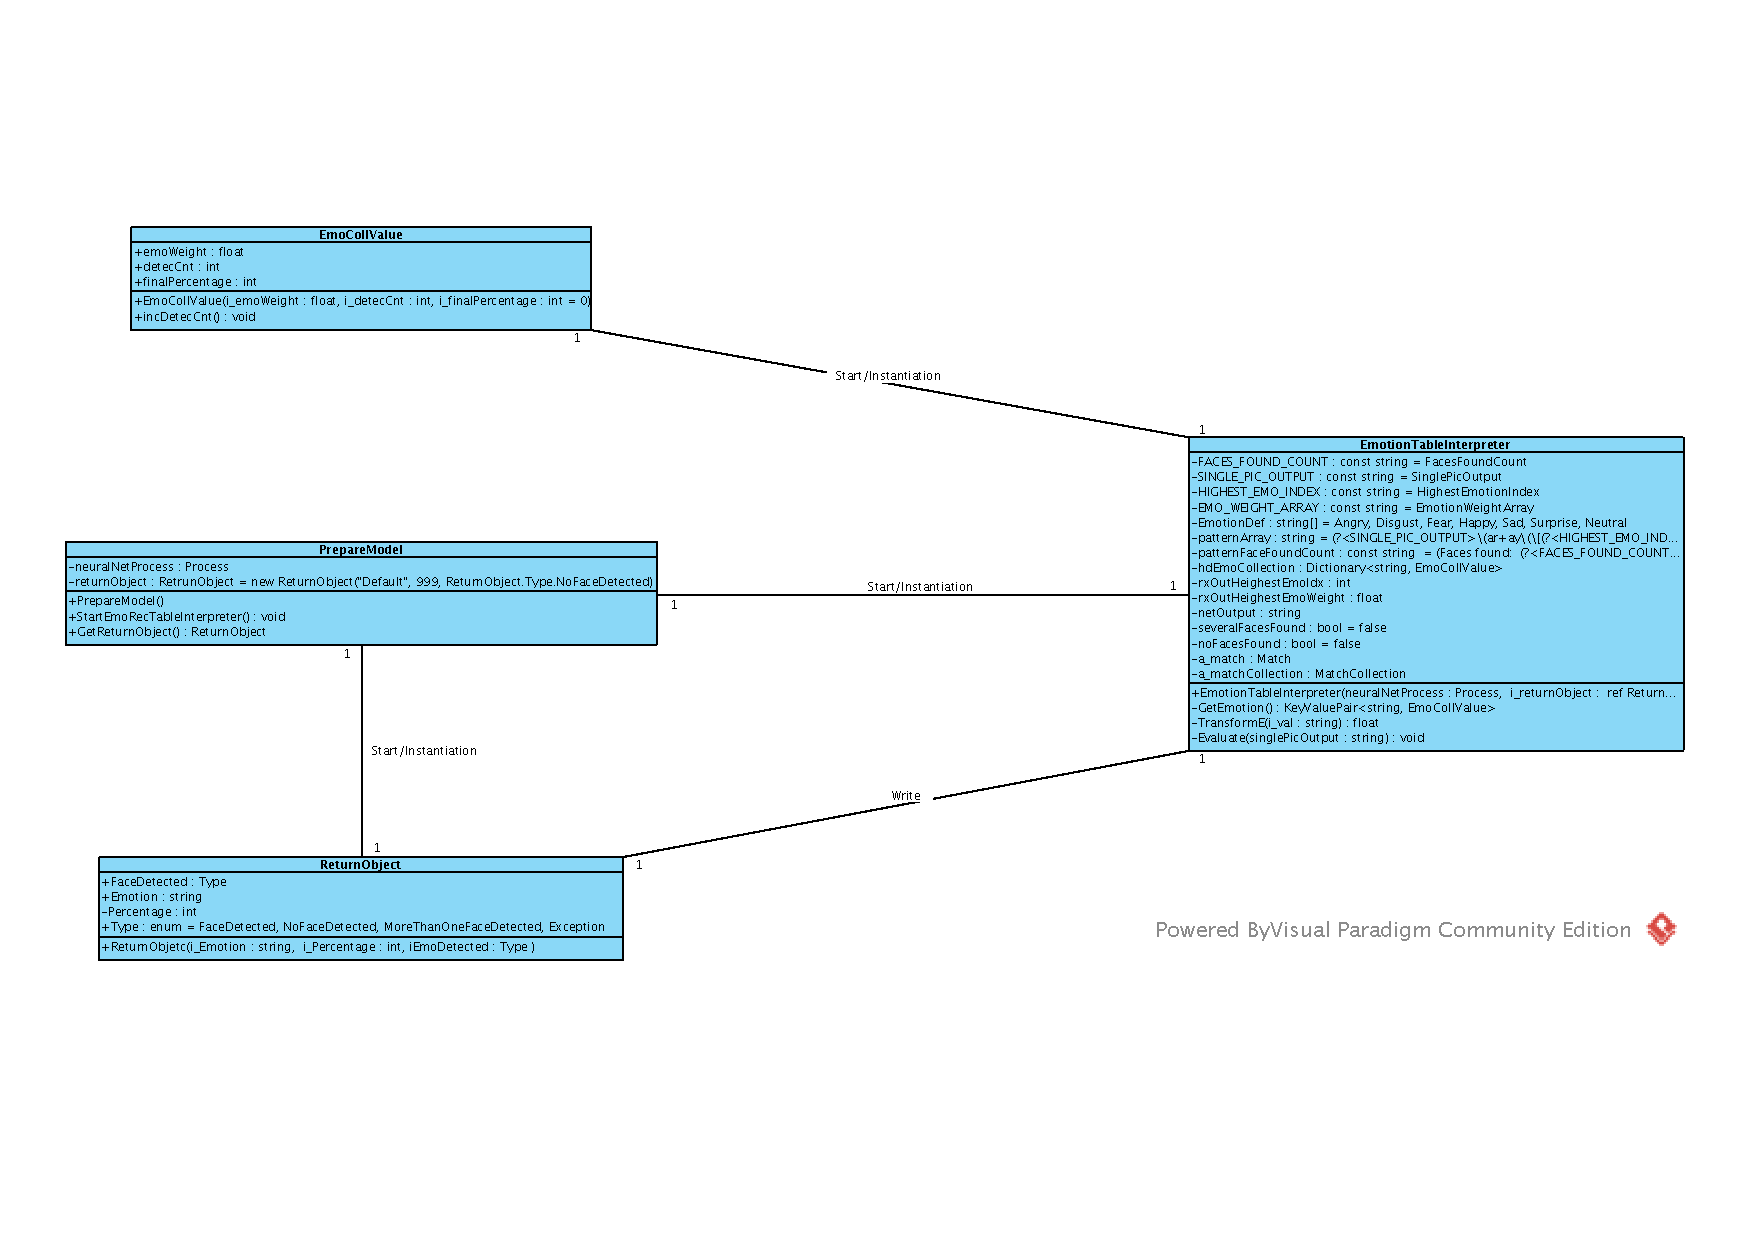
\includegraphics[scale=0.25]{NNUMLFertig.pdf}
% \caption{Klassendiagramm der Emotionserkennung}
% \label{fig:NNUML}
%\end{figure}
%Lukas Schulz 
\section{Ergebnisse}
\subsubsection{Ergebnisse in der Programmierung}
Die Klassen \textit{PrepareModel}, \textit{EmotionTableInterpreter} und \textit{ReturnObject} wurden erstellt und so miteinander verbunden, dass sie einen externen Prozess starten k\"{o}nnen und die Ausgabe dieses Prozesses in den eigenen Prozess einlesen, verarbeiten und weitergeben. Die Klasse \textit{PrepareModel} stellt je ein Objekt der Klassen \textit{System.Diagnostics.Process},  \textit{ReturnObject} und \"{u}bergibt sie einem ebenfalls bereitgestellten Objekt der Klasse  \textit{EmotionTableInterpreter}.

In der Klasse \textit{EmotionTableInterpreter} wird das \textit{System.Diagnostics.Process}-Objekt gestartet. Diese Aktion startet eine Instanz des externen Programms \textit{Python.exe}. In diesem Programm werden vom aufrufenden Programm zur Verf\"{u}gung gestellte Bilder mit Hilfe eines von Lewe Ohlsen \cite{LeweOhlsen} erstellten und trainierten neuronalen Netzes auf der Grundlage des FER+-Trainingsdatensatzes aus. Diese Daten werden als Objekt des Typs \textit{string} wieder in die Klasse \textit{EmotionTableInterpreter} eingelesen und dort von selbst entwickelten regul\"{a}ren Ausdr\"{u}cken mit Hilfe der Systembibliothek \textit{System.Text.RegularExpressions} auf die relevanten Daten untersucht und an das \textit{ReturnObject}-Objekt \"{u}bergeben. Dieses kann dann weiter verarbeitet werden. Teile des in \textit{Python} geschriebenen, zum neuronalen Netz geh\"{o}rigen Skripts wurden auf die Bed\"{u}rfnisse des Programms angepasst. So ruft nun das \textit{Python}-Skript abgespeicherte Bilder auf, anstatt dauernd den Input einer Webcam zu verarbeiten. Zus\"{a}tzlich wurde der Aufruf der GUI des Skripts gel\"{o}scht.
\subsubsection{Ergebnisse in der Verwendung aller Programmteile}
Vor der ersten Ausf\"{u}hrung des Programms m\"{u}ssen mehrere Punkte beachtet werden.
\begin{itemize}
\item[-] Es muss Python 3.6 oder h\"{o}her auf dem Zielger\"{a}t installiert sein.
\item[-] Python muss in die PATH-Variable des Zielger\"{a}tes eingef\"{u}gt worden sein.
\item[-] Das Netz muss wie in der Anleitung\cite{LeweOhlsenGit} von Lewe Ohlsen mit dem Kommandozeilenbefehl \textit{python pip -install -r ''requirements.txt''} installiert werden.
\end{itemize} 
Im Betrieb des Programms fallen verschiedene Besonderheiten mit Bezug zum neuronalen Netz auf, die vor einer Installation bedacht werden sollten.
\begin{itemize}
\item[-] Die ''Positiven'' und die ''neutrale'' Emotion werden am Einfachsten erkannt. ''Negative'' Emotionen werden seltener erkannt.
\item[-] Manchmal werden Gesichter in Strukturen erkannt, die kein Gesicht sind. Verschiedene Experimente konnten keine Struktur hinter diesem Verhalten aufzeigen.
\item[-] Personen, die Brillen tragen m\"{u}ssen diese vor dem Spielstart abnehmen, da die Brillen das Ergebnis der Auswertung ver\"{a}ndern und meistens die ''Emotion'' \textit{''\"{U}berrascht''} erkannt wird. 
\end{itemize}
\section{Diskussion der Ergebnisse}
Im programmierbaren Teil finden sich keine \"{U}berraschungen. Alle Teile der Sprache \textit{C\#} haben wie erwartet miteinander funktioniert und die gew\"{u}nschten Ergebnisse geliefert. Der einfache Aufruf von \textit{Python}-Skripten aus dem Programm heraus war eine erfreuliche \"{U}berraschung, die sehr viel Entwicklungsarbeit ersparte. Die regul\"{a}ren Ausdr\"{u}cke kommen im Allgemeinen nicht sonderlich gut mit im Eingabestring vorhandenen Steuerzeichen zurecht. Dieser Fehler wurde erst in der Testphase erkannt und behoben werden. Der aktuell gew\"{a}hlte Weg ist zwar nicht optimal, entfernt aber Steuerzeichen zuverl\"{a}ssig. Leider war die Ausgabe des mit \textit{CK+} trainierten Models nicht so einfach auswertbar wie die Ausgabe des mit \textit{FER+} trainierten Models. Da \textit{CK+} manchmal als besserer Trainingsdatensatz zur Emotionserkennung eingestuft wird, beeinflu{\ss}t dieses Ereignis die Daten der Auswertung in ihrer Qualit\"{a}t negativ. Vor allem die Erkennung der ''negativen'' Emotionen ist im \textit{CK+}-Datensatz erheblich verbessert.  Nicht \"{u}berraschend waren die Effekte, die erzeugt werden k\"{o}nnen, wenn ein Bild eines Brillentr\"{a}gers ausgewertet wird. Aufgrund der Arbeitsweise des neuronalen Netzes werden Brillen als ''aufgerissene Augen'' erkannt. Das kann ein Nachteil f\"{u}r Brillentr\"{a}ger sein, die den angezeigten Emoji vielleicht nicht erkennen k\"{o}nnen. Solche Nachteile m\"{u}ssen mit einer geschickten Platzierung der Kamera ausgeglichen werden.
\section{Zusammenfassung}
Unser gemeinsames Ziel als NN-Gruppe war es, dem neuronalen Netz von Lewe Ohlsen ein Ger\"{u}st zu geben, mit dem es ohne Probleme von einem \textit{C\#}-Programm aufgerufen und sein Output eingelesen werden kann.%32
Wir verwendeten die M\"{o}lichkeiten, die uns von der Sprachen \textit{C\#} und Python zur Verf\"{u}gung gestellt wurden. Besonders hervorzuheben sind \textit{System.Text.RegularExpressions} und \textit{System.Diagnostics}, welchen den Start, das Auslesen und das Auswerten des Ergebnisses eines von diesem Programm gestarteten Prozesses erm\"{o}lichen. OpenCV und Tensorflow werden genutzt, um die auszuwertenden Bilder vorzubereiten und zu verarbeiten.%51
Es wurden drei Klassen geschrieben, die einen bestimmten externen Prozess starten und auswerten k\"{o}nnen. Das Programm des Prozesses ist in einer anderen Programmiersprache geschrieben und die Ergebnisse m\"{u}ssen von den Klassen als String eingelesen und mit den geeigneten Mitteln ausgewertet werden. Die Ergebnisse des Python-Prozesses h\"{a}ngen in besonderem Ma{\ss}e vom gew\"{a}hlten Model ab. Je nach dem mit welchem Datensatz das Model trainiert wurde, werden Gesichtsausdr\"{u}cke unterschiedlich bewertet und ausgegeben. %68
Die ausgewerteten Daten werden mit regul\"{a}ren Ausdr\"{u}cken verglichen und von geeigneten Funktionen auf die H\"{a}ufigkeit der aufgetretenen Emotion untersucht. Diese Information wird danach in einem Objekt an die aufrufenden Klassen zur\"{u}ckgegeben.%31
\newline
Aufgrund der Daten und der Umsetzung l\"{a}sst sich schlussfolgern, dass das Programm erfolgreich Gesichtsausdr\"{u}cken ''Emotionen'' erfolgreich zuordnen kann und die Ergebnisse dieser Zuordnung an aufrufende Klassen und Programme ausgeben kann.%30
 

\bibliographystyle{plain}
\bibliography{Doku}
%
\end{document}